\documentclass[11pt,a4paper]{article}

\usepackage[utf8]{inputenc}
\usepackage[T1]{fontenc}
\usepackage{mathpazo}
\usepackage[scaled=0.92]{helvet}
\usepackage[margin=1in]{geometry}
\usepackage{graphicx}
\usepackage{amsmath,amssymb,amsfonts}
\usepackage{booktabs}
\usepackage{tabularx}
\usepackage{setspace}
\usepackage{titlesec}
\usepackage{fancyhdr}
\usepackage{float}
\usepackage{caption}
\usepackage{microtype}
\usepackage{tikz}
\usepackage{xcolor}
\usepackage{listings}
\usepackage[hidelinks]{hyperref}

\usetikzlibrary{shapes.geometric, arrows.meta, positioning, calc, matrix, fit, backgrounds}

\setstretch{1.15}
\setlength{\parindent}{0pt}
\setlength{\parskip}{0.8em}
\sloppy

\titleformat{\section}{\normalfont\large\bfseries\sffamily}{\thesection}{1em}{}
\titleformat{\subsection}{\normalfont\normalsize\bfseries\sffamily}{\thesubsection}{1em}{}
\titleformat{\subsubsection}{\normalfont\normalsize\itshape\sffamily}{\thesubsubsection}{1em}{}

\pagestyle{fancy}
\fancyhf{}
\fancyhead[L]{\small\sffamily Fungsi untuk RPL}
\fancyhead[R]{\small\sffamily\thepage}
\renewcommand{\headrulewidth}{0.4pt}

\captionsetup{font=small,labelfont=bf,labelsep=period}

\renewenvironment{abstract}
{\small
	\begin{center}\textbf{\sffamily Abstrak}\end{center}
	\begin{quote}}
	{\end{quote}}

\lstdefinestyle{code}{
	basicstyle=\ttfamily\small,
	frame=single,
	rulecolor=\color{black},
	breaklines=true,
	showstringspaces=false,
	columns=fullflexible,
	keepspaces=true,
	framesep=6pt,
	aboveskip=1em,
	belowskip=1em,
	xleftmargin=0pt
}

\lstdefinestyle{out}{
	basicstyle=\ttfamily\small,
	frame=tb,
	rulecolor=\color{black},
	breaklines=true,
	showstringspaces=false,
	columns=fullflexible,
	keepspaces=true,
	framesep=4pt,
	aboveskip=1em,
	belowskip=1em
}

\title{\vspace{-1.5cm}\textbf{\sffamily\LARGE Fungsi untuk Rekayasa Perangkat Lunak\\ Modul Belajar dengan Visual yang Dapat Dibaca Tanpa Melihat}}
\author{
	\textbf{Muhammad Riduwan Khafidi} \\
	\small Program Studi Teknik Rekayasa Perangkat Lunak \\
	\small Politeknik Negeri Batam \\
	\small \texttt{4342611034@students.polibatam.ac.id}
}
\date{\small\today}

\begin{document}

\maketitle
\thispagestyle{empty}

\begin{abstract}
	Fungsi adalah aturan yang memasangkan setiap anggota daerah asal dengan tepat satu anggota daerah hasil, dan aturan itu menjadi fondasi dari setiap algoritma perangkat lunak. Modul ini membahas definisi fungsi, cara memeriksanya, sifat injektif, surjektif, dan bijektif, invers, komposisi, fungsi khusus seperti lantai, langit-langit, dan modulo, serta fungsi rekursif. Setiap konsep dibuka dengan analogi konkret, dilengkapi contoh berangka yang ditulis langkah demi langkah, dan ditutup dengan tabel ringkas. Sepuluh visual dirancang hitam-putih dan disertai narasi pengganti gambar sehingga pembaca yang mengandalkan teks tetap dapat memahaminya. Modul ini memuat dua belas tabel ringkas, satu studi kasus delapan langkah tentang sandi geser, satu bagian merancang kasus uji, dan tiga prinsip penutup. Setelah membaca modul ini, pembaca dapat memeriksa apakah suatu relasi adalah fungsi, menentukan sifatnya, mencari inversnya, menyambung dua fungsi, menulis fungsi rekursif, dan merancang kasus uji untuk membuktikan kebenarannya.
\end{abstract}

\section{Pendahuluan}

\subsection{Analogi Pembuka: Buku Kontak di Ponsel}

Bayangkan buku kontak di ponsel. Setiap nama punya satu nomor telepon. Jika Ani punya dua nomor, ponsel hanya menyimpan satu sebagai nomor utama, sedangkan nomor lain masuk ke catatan tambahan. Jika Budi belum menyimpan nomor sama sekali, ponsel tidak menampilkan nomor ketika namanya dicari. Jika Citra punya satu nomor, ponsel langsung menampilkan nomor itu.

Buku kontak adalah contoh fungsi. Setiap nama dipasangkan dengan tepat satu nomor. Nama tanpa nomor adalah masukan yang belum punya hasil. Nama dengan dua nomor adalah masukan yang hasilnya lebih dari satu, dan itu bukan fungsi.

Fungsi adalah aturan yang menjamin satu jawaban pasti untuk setiap masukan. Jaminan itu yang membuat program dapat memberi hasil yang dapat diuji.

\subsection{Mengapa Topik Ini Penting}

Setiap algoritma adalah fungsi. Fungsi sortir memasangkan setiap larik masukan dengan satu larik terurut. Fungsi hash memasangkan setiap teks dengan satu bilangan. Fungsi enkripsi memasangkan setiap pesan dengan satu pesan rahasia.

Tanpa teori fungsi, pengembang sulit menjawab pertanyaan yang tampaknya sepele. Mengapa fungsi harus mengembalikan satu nilai, bukan dua? Mengapa fungsi yang sama dengan masukan sama harus memberi hasil sama? Mengapa enkripsi bisa didekripsi tetapi hash tidak bisa? Semua jawaban itu berasal dari sifat-sifat fungsi \cite{rosen}.

\subsection{Cara Membaca Modul Ini}

Setiap bagian mengikuti pola yang sama. Pertama, analogi konkret. Kedua, definisi formal. Ketiga, contoh berangka yang ditulis langkah demi langkah. Keempat, visual dengan narasi pengganti gambar. Kelima, tabel ringkas. Setiap konsep kunci diberi dua bagian tambahan: Cara Berpikir yang menjelaskan langkah mental menyelesaikan soal, dan Kalau Salah yang menunjukkan akibat jika langkah dilewati.

\subsection{Peta Pembahasan}

Bagian kedua membahas definisi fungsi dan tiga kasus kampus. Bagian ketiga membahas cara memeriksa fungsi. Bagian keempat membahas sifat fungsi. Bagian kelima membahas invers. Bagian keenam membahas komposisi. Bagian ketujuh membahas fungsi khusus. Bagian kedelapan membahas fungsi rekursif. Bagian kesembilan menyandingkan seluruh konsep. Bagian kesepuluh memakai konsep pada studi kasus sandi geser. Bagian kesebelas membahas perancangan kasus uji. Bagian keduabelas dan ketigabelas memberi daftar kesalahan umum dan lembar rujukan cepat. Bagian keempatbelas menutup dengan tiga prinsip.

\section{Definisi Fungsi}

\subsection{Analogi: Mesin Bubur}

Bayangkan mesin bubur di kantin. Mesin itu punya satu lubang masukan dan satu lubang keluaran. Ketika kita memasukkan satu bungkus beras, mesin mengeluarkan satu mangkuk bubur. Ketika kita memasukkan satu bungkus kacang hijau, mesin mengeluarkan satu mangkuk bubur kacang hijau. Namun jika kita memasukkan satu bungkus beras dan mesin mengeluarkan dua mangkuk bubur sekaligus, itu bukan mesin yang bisa diandalkan.

Fungsi bekerja seperti mesin itu. Setiap masukan menghasilkan tepat satu keluaran. Mesin yang menghasilkan lebih dari satu keluaran tidak memenuhi syarat fungsi.

\subsection{Definisi Formal}

Fungsi $f$ dari himpunan $A$ ke himpunan $B$ adalah aturan yang memasangkan setiap anggota $A$ dengan tepat satu anggota $B$. Notasinya $f:A \to B$, dan hasil pemetaan $a$ ditulis $f(a)=b$ yang dibaca "f dari a sama dengan b" \cite{rosen}.

Tiga istilah yang perlu dibedakan. Daerah asal atau domain adalah himpunan semua masukan, yaitu $A$. Kodomain adalah himpunan tempat hasil boleh berada, yaitu $B$. Jelajah atau range adalah himpunan hasil yang benar-benar muncul, yaitu himpunan semua $f(a)$ untuk $a \in A$.

Perhatikan bahwa jelajah adalah himpunan bagian dari kodomain. Kodomain boleh memuat anggota yang tidak pernah menjadi hasil. Jelajah hanya memuat hasil yang benar-benar muncul.

\subsection{Tiga Kasus Data Kampus}

Tiga kasus dari data kampus memperjelas perbedaan antara bukan fungsi, fungsi, dan fungsi parsial. Perhatikan Tabel~\ref{tab:tiga-kasus} dan Gambar~\ref{fig:tiga-kasus}.

\begin{table}[H]
	\centering
	\caption{Tiga kasus data kampus dan status fungsinya.}
	\label{tab:tiga-kasus}
	\small
	\begin{tabularx}{\textwidth}{l X X}
		\toprule
		Data                     & Contoh pasangan                       & Status                               \\
		\midrule
		Mata kuliah diambil      & $M3 \to MTK$ dan $M3 \to RPL$         & bukan fungsi, M3 punya dua hasil     \\
		Dosen wali lengkap       & $M1 \to D1$, $M2 \to D2$, $M3 \to D1$ & fungsi                               \\
		Dosen wali belum lengkap & $M1 \to D1$, $M2 \to D2$              & fungsi parsial, M3 belum punya hasil \\
		\bottomrule
	\end{tabularx}
\end{table}

\begin{figure}[H]
	\centering
	\resizebox{\textwidth}{!}{%
		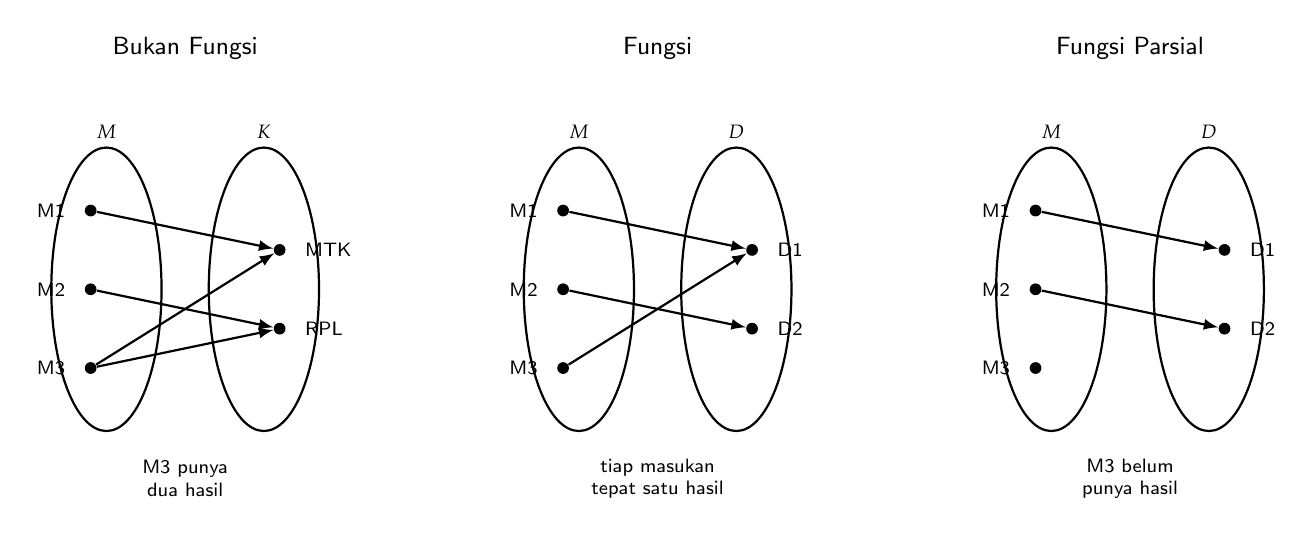
\begin{tikzpicture}[
				dot/.style={circle, fill=black, inner sep=1.5pt},
				elbl/.style={font=\scriptsize\sffamily},
				hdr/.style={font=\sffamily\small, anchor=south}
			]
			\begin{scope}[shift={(-6, 0)}]
				\node[hdr] at (1, 2.8) {Bukan Fungsi};
				\draw[thick] (0, 0) ellipse (0.7 and 1.8);
				\draw[thick] (2, 0) ellipse (0.7 and 1.8);
				\node[elbl] at (0, 2.0) {$M$};
				\node[elbl] at (2, 2.0) {$K$};
				\node[dot] (m1) at (-0.2, 1.0) {};
				\node[dot] (m2) at (-0.2, 0) {};
				\node[dot] (m3) at (-0.2, -1.0) {};
				\node[elbl, anchor=east] at (-0.4, 1.0) {M1};
				\node[elbl, anchor=east] at (-0.4, 0) {M2};
				\node[elbl, anchor=east] at (-0.4, -1.0) {M3};
				\node[dot] (k1) at (2.2, 0.5) {};
				\node[dot] (k2) at (2.2, -0.5) {};
				\node[elbl, anchor=west] at (2.4, 0.5) {MTK};
				\node[elbl, anchor=west] at (2.4, -0.5) {RPL};
				\draw[thick, -latex] (m1) -- (k1);
				\draw[thick, -latex] (m2) -- (k2);
				\draw[thick, -latex] (m3) -- (k1);
				\draw[thick, -latex] (m3) -- (k2);
				\node[font=\scriptsize\sffamily, align=center] at (1, -2.4) {M3 punya\\dua hasil};
			\end{scope}
			\begin{scope}[shift={(0, 0)}]
				\node[hdr] at (1, 2.8) {Fungsi};
				\draw[thick] (0, 0) ellipse (0.7 and 1.8);
				\draw[thick] (2, 0) ellipse (0.7 and 1.8);
				\node[elbl] at (0, 2.0) {$M$};
				\node[elbl] at (2, 2.0) {$D$};
				\node[dot] (m1) at (-0.2, 1.0) {};
				\node[dot] (m2) at (-0.2, 0) {};
				\node[dot] (m3) at (-0.2, -1.0) {};
				\node[elbl, anchor=east] at (-0.4, 1.0) {M1};
				\node[elbl, anchor=east] at (-0.4, 0) {M2};
				\node[elbl, anchor=east] at (-0.4, -1.0) {M3};
				\node[dot] (d1) at (2.2, 0.5) {};
				\node[dot] (d2) at (2.2, -0.5) {};
				\node[elbl, anchor=west] at (2.4, 0.5) {D1};
				\node[elbl, anchor=west] at (2.4, -0.5) {D2};
				\draw[thick, -latex] (m1) -- (d1);
				\draw[thick, -latex] (m2) -- (d2);
				\draw[thick, -latex] (m3) -- (d1);
				\node[font=\scriptsize\sffamily, align=center] at (1, -2.4) {tiap masukan\\tepat satu hasil};
			\end{scope}
			\begin{scope}[shift={(6, 0)}]
				\node[hdr] at (1, 2.8) {Fungsi Parsial};
				\draw[thick] (0, 0) ellipse (0.7 and 1.8);
				\draw[thick] (2, 0) ellipse (0.7 and 1.8);
				\node[elbl] at (0, 2.0) {$M$};
				\node[elbl] at (2, 2.0) {$D$};
				\node[dot] (m1) at (-0.2, 1.0) {};
				\node[dot] (m2) at (-0.2, 0) {};
				\node[dot] (m3) at (-0.2, -1.0) {};
				\node[elbl, anchor=east] at (-0.4, 1.0) {M1};
				\node[elbl, anchor=east] at (-0.4, 0) {M2};
				\node[elbl, anchor=east] at (-0.4, -1.0) {M3};
				\node[dot] (d1) at (2.2, 0.5) {};
				\node[dot] (d2) at (2.2, -0.5) {};
				\node[elbl, anchor=west] at (2.4, 0.5) {D1};
				\node[elbl, anchor=west] at (2.4, -0.5) {D2};
				\draw[thick, -latex] (m1) -- (d1);
				\draw[thick, -latex] (m2) -- (d2);
				\node[font=\scriptsize\sffamily, align=center] at (1, -2.4) {M3 belum\\punya hasil};
			\end{scope}
		\end{tikzpicture}}
	\caption{Tiga kasus data kampus: bukan fungsi, fungsi, dan fungsi parsial.}
	\label{fig:tiga-kasus}
\end{figure}

Cara membaca Gambar~\ref{fig:tiga-kasus}: gambar ini terdiri dari tiga panel dari kiri ke kanan. Panel pertama berjudul "Bukan Fungsi" dan menampilkan elips $M$ berisi tiga titik M1, M2, M3 serta elips $K$ berisi dua titik MTK dan RPL. Ada empat panah: M1 ke MTK, M2 ke RPL, dan M3 bercabang ke MTK dan RPL sekaligus. Di bawah panel tertulis "M3 punya dua hasil". Panel kedua berjudul "Fungsi" dan menampilkan elips $M$ dan elips $D$. Ada tiga panah, masing-masing dari satu mahasiswa ke satu dosen. M1 dan M3 sama-sama mengarah ke D1, sedangkan M2 ke D2. Di bawah panel tertulis "tiap masukan tepat satu hasil". Panel ketiga berjudul "Fungsi Parsial" dan menampilkan elips $M$ dan $D$ dengan hanya dua panah: M1 ke D1 dan M2 ke D2. Titik M3 tidak punya panah keluar. Di bawah panel tertulis "M3 belum punya hasil". Inti pesan gambar ini adalah perbedaan kunci antara tiga kasus terletak pada jumlah panah keluar dari setiap masukan.

\subsection{Cara Berpikir: Memeriksa Apakah Relasi adalah Fungsi}

Untuk memeriksa apakah suatu relasi adalah fungsi, ajukan tiga pertanyaan secara berurutan. Pertama, apa saja masukannya? Tuliskan seluruh domain. Kedua, untuk setiap masukan, hitung berapa hasil yang dimilikinya. Jika ada masukan dengan dua hasil atau lebih, relasi itu bukan fungsi. Ketiga, apakah ada masukan tanpa hasil? Jika ada, relasi itu fungsi parsial, bukan fungsi lengkap.

Jika ketiga pertanyaan itu dijawab, status relasi sudah pasti. Tidak perlu menebak.

\subsection{Kalau Salah: Mengira Semua Relasi adalah Fungsi}

Kesalahan paling sering adalah mengira setiap relasi adalah fungsi. Relasi "M3 mengambil MTK dan M3 mengambil RPL" bukan fungsi, karena M3 punya dua hasil. Relasi ini adalah relasi biasa, tetapi bukan fungsi.

Kesalahan ini berbahaya di pemrograman. Jika pengembang menganggap relasi seperti itu sebagai fungsi dan menulis kode yang mengembalikan satu nilai, kode itu akan mengembalikan salah satu hasil secara sembarang. Bug ini sulit ditemukan karena kadang-kadang hasilnya benar, tergantung urutan data di memori.

\subsection{Mengapa Ini Penting}

Basis data relasional membedakan relasi biasa dan fungsi. Relasi biasa boleh memiliki banyak hasil per masukan, sedangkan fungsi hanya boleh memiliki satu. Kolom foreign key yang unik (unique constraint) memaksa relasi menjadi fungsi, karena setiap masukan hanya boleh muncul satu kali. Kolom foreign key tanpa unique constraint membiarkan relasi menjadi relasi biasa. Pilihan constraint ini didasarkan pada pemahaman fungsi \cite{silberschatz}.

\subsection{Ringkasan}

Tabel~\ref{tab:fungsi-relasi} merangkum perbedaan fungsi dan relasi biasa.

\begin{table}[H]
	\centering
	\caption{Perbandingan fungsi dan relasi biasa.}
	\label{tab:fungsi-relasi}
	\small
	\begin{tabularx}{\textwidth}{l X X}
		\toprule
		Aspek               & Relasi biasa             & Fungsi             \\
		\midrule
		Hasil per masukan   & boleh lebih dari satu    & tepat satu         \\
		Masukan tanpa hasil & boleh                    & fungsi parsial     \\
		Contoh kampus       & M3 mengambil MTK dan RPL & M1 dosen wali D1   \\
		Padanan SQL         & foreign key biasa        & foreign key unique \\
		\bottomrule
	\end{tabularx}
\end{table}

\section{Cara Memeriksa Fungsi}

\subsection{Tiga Pertanyaan}

Untuk memeriksa fungsi dari sisi masukan, ajukan tiga pertanyaan. Pertama, apa saja masukannya? Ini menentukan domain. Kedua, tiap masukan punya berapa hasil? Jika ada yang lebih dari satu, bukan fungsi. Ketiga, ada masukan tanpa hasil? Jika ada, fungsi itu parsial.

Ketiga pertanyaan itu bisa dijawab dari daftar pasangan tanpa perlu menggambar. Cukup hitung berapa kali setiap masukan muncul sebagai komponen pertama.

\subsection{Analogi Buku Kontak}

Buku kontak di ponsel memuat pasangan nama dan nomor. Ani dengan satu nomor adalah fungsi lengkap untuk Ani. Budi tanpa nomor adalah fungsi parsial untuk Budi. Citra dengan dua nomor utama adalah bukan fungsi untuk Citra.

Ketiga keadaan itu memetakan persis ke tiga pertanyaan sebelumnya.

\subsection{Dalam Program}

Di Python, kamus (dictionary) adalah implementasi fungsi. Kunci adalah masukan, nilai adalah hasil. Setiap kunci hanya boleh muncul satu kali. Akses ke kunci yang tidak ada menghasilkan galat KeyError, yang setara dengan masukan tanpa hasil pada fungsi parsial.

Contoh: kamus \texttt{nilai~=~\{"M1":~80,~"M2":~75\}}. Akses \texttt{nilai["M1"]} mengembalikan 80. Akses \texttt{nilai["M3"]} mengembalikan galat. Akses \texttt{nilai["M1"]~=~85} akan menimpa nilai lama, karena kunci hanya boleh muncul satu kali.

\section{Sifat Fungsi}

\subsection{Analogi: Tiga Jenis Pengiriman}

Bayangkan tiga jenis pengiriman surat. Pengiriman pertama menjamin setiap alamat hanya menerima satu surat, tetapi tidak semua alamat kebagian surat. Pengiriman kedua menjamin setiap alamat kebagian surat, tetapi mungkin ada alamat yang menerima lebih dari satu surat. Pengiriman ketiga menjamin setiap alamat kebagian tepat satu surat, tidak lebih dan tidak kurang.

Ketiga jaminan itu adalah injektif, surjektif, dan bijektif.

\subsection{Injektif}

Fungsi $f:A \to B$ disebut injektif jika tidak ada dua masukan berbeda yang hasilnya sama. Dengan kata lain, jika $f(a_1)=f(a_2)$, maka $a_1=a_2$. Syarat perlu: $|A| \le |B|$, karena setiap masukan harus mendapat hasil berbeda, sehingga hasil yang tersedia minimal sebanyak masukan \cite{rosen}.

Contoh: $f(x)=x^2$ pada bilangan real bukan injektif, karena $f(3)=9$ dan $f(-3)=9$ walaupun $3 \ne -3$. Contoh injektif di perangkat lunak: NIM mahasiswa, karena tidak ada dua mahasiswa dengan NIM sama.

\subsection{Surjektif}

Fungsi $f:A \to B$ disebut surjektif jika setiap anggota $B$ menjadi hasil dari minimal satu masukan. Syarat perlu: $|A| \ge |B|$, karena setiap anggota kodomain harus kebagian hasil.

Contoh: $f(x)=x+1$ pada bilangan real surjektif, karena setiap bilangan $r$ di kodomain berasal dari $r-1$ di domain. Di perangkat lunak, contoh surjektif adalah fungsi yang memetakan setiap ID pesanan ke salah satu status pesanan yang mungkin, dengan jaminan setiap status pernah dicapai.

\subsection{Bijektif}

Fungsi $f:A \to B$ disebut bijektif jika injektif sekaligus surjektif. Setiap masukan mendapat hasil berbeda, dan setiap anggota kodomain kebagian tepat satu hasil. Hanya fungsi bijektif yang punya invers \cite{rosen}.

Contoh: $f(x)=x+1$ pada bilangan real bijektif. Di perangkat lunak, contoh bijektif adalah enkripsi dan dekripsi. Enkripsi memetakan setiap pesan asli ke tepat satu pesan rahasia, dan dekripsi memetakan balik.

Perhatikan Gambar~\ref{fig:sifat-fungsi} yang menyandingkan ketiga sifat.

\begin{figure}[H]
	\centering
	\resizebox{\textwidth}{!}{%
		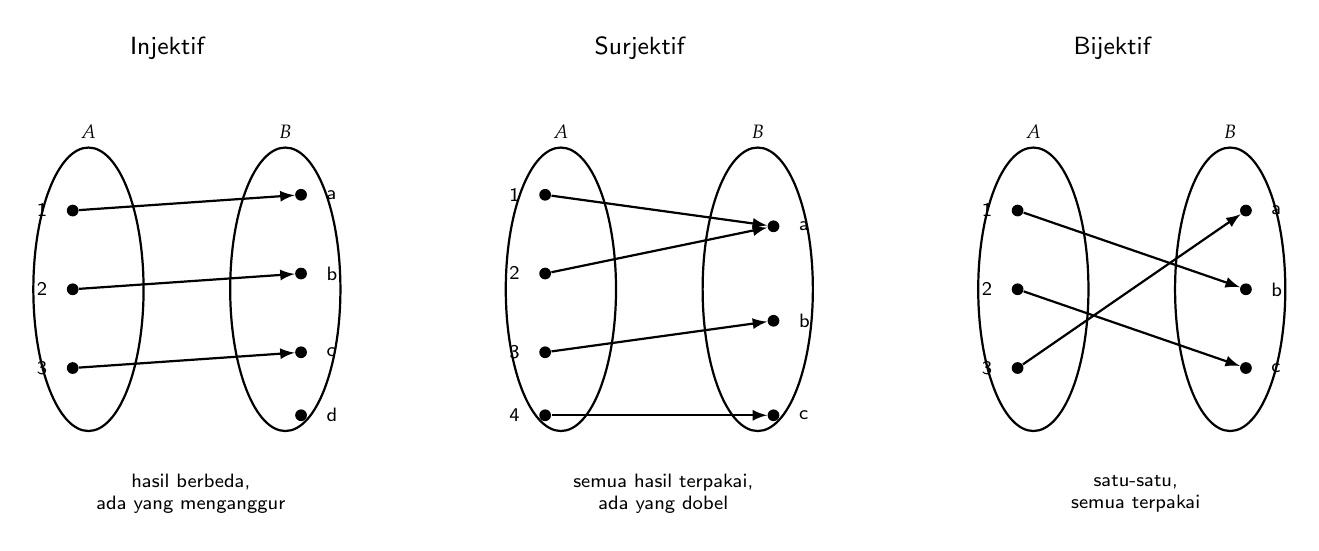
\begin{tikzpicture}[
				dot/.style={circle, fill=black, inner sep=1.5pt},
				elbl/.style={font=\scriptsize\sffamily},
				hdr/.style={font=\sffamily\small, anchor=south}
			]
			\begin{scope}[shift={(-6, 0)}]
				\node[hdr] at (1, 2.8) {Injektif};
				\draw[thick] (0, 0) ellipse (0.7 and 1.8);
				\draw[thick] (2.5, 0) ellipse (0.7 and 1.8);
				\node[elbl] at (0, 2.0) {$A$};
				\node[elbl] at (2.5, 2.0) {$B$};
				\node[dot] (a1) at (-0.2, 1.0) {};
				\node[dot] (a2) at (-0.2, 0) {};
				\node[dot] (a3) at (-0.2, -1.0) {};
				\node[elbl, anchor=east] at (-0.4, 1.0) {1};
				\node[elbl, anchor=east] at (-0.4, 0) {2};
				\node[elbl, anchor=east] at (-0.4, -1.0) {3};
				\node[dot] (b1) at (2.7, 1.2) {};
				\node[dot] (b2) at (2.7, 0.2) {};
				\node[dot] (b3) at (2.7, -0.8) {};
				\node[dot] (b4) at (2.7, -1.6) {};
				\node[elbl, anchor=west] at (2.9, 1.2) {a};
				\node[elbl, anchor=west] at (2.9, 0.2) {b};
				\node[elbl, anchor=west] at (2.9, -0.8) {c};
				\node[elbl, anchor=west] at (2.9, -1.6) {d};
				\draw[thick, -latex] (a1) -- (b1);
				\draw[thick, -latex] (a2) -- (b2);
				\draw[thick, -latex] (a3) -- (b3);
				\node[font=\scriptsize\sffamily, align=center] at (1.3, -2.6) {hasil berbeda,\\ada yang menganggur};
			\end{scope}
			\begin{scope}[shift={(0, 0)}]
				\node[hdr] at (1, 2.8) {Surjektif};
				\draw[thick] (0, 0) ellipse (0.7 and 1.8);
				\draw[thick] (2.5, 0) ellipse (0.7 and 1.8);
				\node[elbl] at (0, 2.0) {$A$};
				\node[elbl] at (2.5, 2.0) {$B$};
				\node[dot] (a1) at (-0.2, 1.2) {};
				\node[dot] (a2) at (-0.2, 0.2) {};
				\node[dot] (a3) at (-0.2, -0.8) {};
				\node[dot] (a4) at (-0.2, -1.6) {};
				\node[elbl, anchor=east] at (-0.4, 1.2) {1};
				\node[elbl, anchor=east] at (-0.4, 0.2) {2};
				\node[elbl, anchor=east] at (-0.4, -0.8) {3};
				\node[elbl, anchor=east] at (-0.4, -1.6) {4};
				\node[dot] (b1) at (2.7, 0.8) {};
				\node[dot] (b2) at (2.7, -0.4) {};
				\node[dot] (b3) at (2.7, -1.6) {};
				\node[elbl, anchor=west] at (2.9, 0.8) {a};
				\node[elbl, anchor=west] at (2.9, -0.4) {b};
				\node[elbl, anchor=west] at (2.9, -1.6) {c};
				\draw[thick, -latex] (a1) -- (b1);
				\draw[thick, -latex] (a2) -- (b1);
				\draw[thick, -latex] (a3) -- (b2);
				\draw[thick, -latex] (a4) -- (b3);
				\node[font=\scriptsize\sffamily, align=center] at (1.3, -2.6) {semua hasil terpakai,\\ada yang dobel};
			\end{scope}
			\begin{scope}[shift={(6, 0)}]
				\node[hdr] at (1, 2.8) {Bijektif};
				\draw[thick] (0, 0) ellipse (0.7 and 1.8);
				\draw[thick] (2.5, 0) ellipse (0.7 and 1.8);
				\node[elbl] at (0, 2.0) {$A$};
				\node[elbl] at (2.5, 2.0) {$B$};
				\node[dot] (a1) at (-0.2, 1.0) {};
				\node[dot] (a2) at (-0.2, 0) {};
				\node[dot] (a3) at (-0.2, -1.0) {};
				\node[elbl, anchor=east] at (-0.4, 1.0) {1};
				\node[elbl, anchor=east] at (-0.4, 0) {2};
				\node[elbl, anchor=east] at (-0.4, -1.0) {3};
				\node[dot] (b1) at (2.7, 1.0) {};
				\node[dot] (b2) at (2.7, 0) {};
				\node[dot] (b3) at (2.7, -1.0) {};
				\node[elbl, anchor=west] at (2.9, 1.0) {a};
				\node[elbl, anchor=west] at (2.9, 0) {b};
				\node[elbl, anchor=west] at (2.9, -1.0) {c};
				\draw[thick, -latex] (a1) -- (b2);
				\draw[thick, -latex] (a2) -- (b3);
				\draw[thick, -latex] (a3) -- (b1);
				\node[font=\scriptsize\sffamily, align=center] at (1.3, -2.6) {satu-satu,\\semua terpakai};
			\end{scope}
		\end{tikzpicture}}
	\caption{Perbandingan sifat injektif, surjektif, dan bijektif pada diagram panah.}
	\label{fig:sifat-fungsi}
\end{figure}

Cara membaca Gambar~\ref{fig:sifat-fungsi}: gambar ini menampilkan tiga panel dari kiri ke kanan. Panel pertama berjudul "Injektif" dan menampilkan elips $A$ dengan tiga masukan dan elips $B$ dengan empat hasil. Tiga panah keluar dari masukan ke tiga hasil berbeda, sedangkan satu hasil di kanan tidak punya panah masuk. Di bawah panel tertulis "hasil berbeda, ada yang menganggur". Panel kedua berjudul "Surjektif" dan menampilkan elips $A$ dengan empat masukan dan elips $B$ dengan tiga hasil. Empat panah keluar, dua di antaranya mengarah ke hasil yang sama, dan semua hasil di kanan kebagian panah. Di bawah panel tertulis "semua hasil terpakai, ada yang dobel". Panel ketiga berjudul "Bijektif" dan menampilkan elips $A$ dengan tiga masukan dan elips $B$ dengan tiga hasil. Tiga panah keluar, satu-satu, semua hasil kebagian tepat satu panah. Di bawah panel tertulis "satu-satu, semua terpakai". Inti pesan gambar ini adalah injektif berbicara tentang masukan, surjektif berbicara tentang hasil, dan bijektif memenuhi keduanya.

\subsection{Latihan Menentukan Sifat}

Tabel~\ref{tab:latihan-sifat} memuat tiga fungsi latihan dengan sifat masing-masing.

\begin{table}[H]
	\centering
	\caption{Latihan menentukan sifat fungsi.}
	\label{tab:latihan-sifat}
	\footnotesize
	\begin{tabularx}{\textwidth}{l c c X}
		\toprule
		Fungsi                          & Injektif & Surjektif & Alasan                                     \\
		\midrule
		$f_1:\{1,2,3,4\} \to \{a,b,c\}$ & tidak    & ya        & 3 dan 4 sama-sama ke c                     \\
		$f_2:\{1,2,3\} \to \{a,b,c,d\}$ & ya       & tidak     & tidak ada panah ke d                       \\
		$f_3:\{1,2,3\} \to \{a,b,c\}$   & ya       & ya        & tiap anggota $B$ menerima tepat satu panah \\
		\bottomrule
	\end{tabularx}
\end{table}

Cek cepat yang sering dipakai: injektif membutuhkan $|A| \le |B|$, surjektif membutuhkan $|A| \ge |B|$. Syarat ini perlu tetapi belum cukup, jadi tetap periksa pasangannya.

\subsection{Cara Berpikir: Memilih Sifat yang Ingin Diperiksa}

Saat memeriksa sifat fungsi, ajukan tiga pertanyaan secara berurutan. Pertama, apakah ada dua masukan berbeda yang hasilnya sama? Jika ya, tidak injektif. Kedua, apakah ada hasil yang tidak pernah muncul? Jika ya, tidak surjektif. Ketiga, apakah injektif sekaligus surjektif? Jika ya, bijektif.

Ketiga pertanyaan itu tidak harus dijawab bersamaan. Jika yang ingin diperiksa hanya injektif, cukup pertanyaan pertama. Jika yang ingin diperiksa invers, cukup pertanyaan ketiga.

\subsection{Ringkasan}

Tabel~\ref{tab:sifat-fungsi} merangkum ketiga sifat.

\begin{table}[H]
	\centering
	\caption{Ringkasan sifat fungsi.}
	\label{tab:sifat-fungsi}
	\small
	\begin{tabularx}{\textwidth}{l X X}
		\toprule
		Sifat     & Arti                              & Padanan di perangkat lunak  \\
		\midrule
		Injektif  & tidak ada dua masukan hasil sama  & NIM unik                    \\
		Surjektif & setiap anggota $B$ kebagian hasil & semua status pernah dicapai \\
		Bijektif  & injektif dan surjektif            & enkripsi dan dekripsi       \\
		\bottomrule
	\end{tabularx}
\end{table}

\section{Invers Fungsi}

\subsection{Analogi: Membalik Resep}

Bayangkan sebuah resep yang mengubah tepung menjadi roti. Jika kita punya roti, bisakah kita menemukan tepung yang dipakai? Jika resepnya bijektif, jawabannya bisa. Jika tidak, jawabannya tidak tunggal.

Invers fungsi membalik arah panah. Setiap hasil dikembalikan ke masukan asal. Jika fungsi $f$ memetakan $a$ ke $b$, maka $f^{-1}$ memetakan $b$ ke $a$. Perhatikan Gambar~\ref{fig:invers-fungsi}.

\begin{figure}[H]
	\centering
	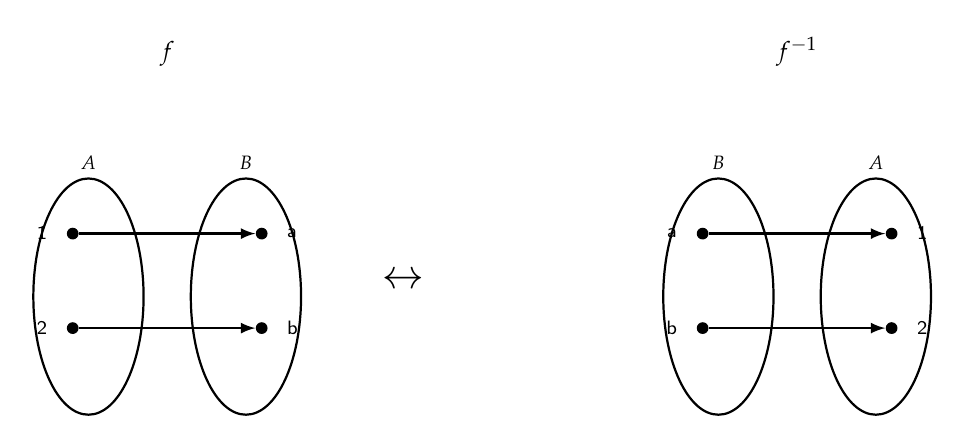
\begin{tikzpicture}[
			dot/.style={circle, fill=black, inner sep=1.5pt},
			elbl/.style={font=\scriptsize\sffamily},
			hdr/.style={font=\sffamily\small, anchor=south}
		]
		\begin{scope}[shift={(-4, 0)}]
			\node[hdr] at (1, 2.8) {$f$};
			\draw[thick] (0, 0) ellipse (0.7 and 1.5);
			\draw[thick] (2, 0) ellipse (0.7 and 1.5);
			\node[elbl] at (0, 1.7) {$A$};
			\node[elbl] at (2, 1.7) {$B$};
			\node[dot] (a1) at (-0.2, 0.8) {};
			\node[dot] (a2) at (-0.2, -0.4) {};
			\node[elbl, anchor=east] at (-0.4, 0.8) {1};
			\node[elbl, anchor=east] at (-0.4, -0.4) {2};
			\node[dot] (b1) at (2.2, 0.8) {};
			\node[dot] (b2) at (2.2, -0.4) {};
			\node[elbl, anchor=west] at (2.4, 0.8) {a};
			\node[elbl, anchor=west] at (2.4, -0.4) {b};
			\draw[thick, -latex] (a1) -- (b1);
			\draw[thick, -latex] (a2) -- (b2);
		\end{scope}

		\node[font=\Large\sffamily] at (0, 0.2) {$\leftrightarrow$};

		\begin{scope}[shift={(4, 0)}]
			\node[hdr] at (1, 2.8) {$f^{-1}$};
			\draw[thick] (0, 0) ellipse (0.7 and 1.5);
			\draw[thick] (2, 0) ellipse (0.7 and 1.5);
			\node[elbl] at (0, 1.7) {$B$};
			\node[elbl] at (2, 1.7) {$A$};
			\node[dot] (b1) at (-0.2, 0.8) {};
			\node[dot] (b2) at (-0.2, -0.4) {};
			\node[elbl, anchor=east] at (-0.4, 0.8) {a};
			\node[elbl, anchor=east] at (-0.4, -0.4) {b};
			\node[dot] (a1) at (2.2, 0.8) {};
			\node[dot] (a2) at (2.2, -0.4) {};
			\node[elbl, anchor=west] at (2.4, 0.8) {1};
			\node[elbl, anchor=west] at (2.4, -0.4) {2};
			\draw[thick, -latex] (b1) -- (a1);
			\draw[thick, -latex] (b2) -- (a2);
		\end{scope}
	\end{tikzpicture}
	\caption{Fungsi $f$ dan inversnya $f^{-1}$: posisi himpunan ditukar dan arah panah dibalik.}
	\label{fig:invers-fungsi}
\end{figure}

Cara membaca Gambar~\ref{fig:invers-fungsi}: gambar ini menampilkan dua subgambar berdampingan yang dihubungkan tanda panah bolak-balik. Subgambar kiri berjudul $f$ dan menampilkan elips $A$ di kiri dan elips $B$ di kanan. Ada dua panah dari 1 ke a dan dari 2 ke b. Subgambar kanan berjudul $f^{-1}$ dan menampilkan elips $B$ di kiri dan elips $A$ di kanan. Ada dua panah dari a ke 1 dan dari b ke 2. Posisi elips ditukar dan arah panah dibalik. Isi himpunan tetap sama. Inti pesan gambar ini adalah invers fungsi hanya membalik arah, bukan mengubah anggota yang terhubung.

\subsection{Syarat Invers}

Invers fungsi ada jika dan hanya jika fungsi itu bijektif. Fungsi injektif tetapi tidak surjektif tidak punya invers lengkap, karena ada anggota kodomain yang tidak punya pasangan asal. Fungsi surjektif tetapi tidak injektif tidak punya invers tunggal, karena satu hasil bisa berasal dari dua masukan berbeda \cite{rosen}.

\subsection{Langkah Mencari Invers}

Untuk fungsi yang dinyatakan dengan rumus, invers dicari dengan lima langkah. Pertama, pastikan fungsi bijektif. Kedua, tulis $y=f(x)$. Ketiga, cari $x$ dalam $y$. Keempat, ganti $y$ menjadi $x$. Kelima, uji dengan satu angka.

Contoh: $f(x)=2x+3$. Tulis $y=2x+3$. Cari $x$: $2x=y-3$, sehingga $x=(y-3)/2$. Ganti $y$ menjadi $x$: $f^{-1}(x)=(x-3)/2$. Uji dengan satu angka: $f(5)=13$, dan $f^{-1}(13)=(13-3)/2=5$. Cocok.

\subsection{Peringatan: Fungsi yang Tidak Punya Invers}

$f(x)=x^2$ tidak punya invers pada bilangan real. Jika hasilnya 9, nilai asalnya bisa 3 atau $-3$. Ada dua kemungkinan, sehingga invers tidak tunggal. Untuk membuat invers ada, daerah asal harus dibatasi, misalnya $x \ge 0$. Dengan batasan itu, $f^{-1}(x)=\sqrt{x}$ menjadi fungsi yang sah.

Di pemrograman, pembatasan daerah asal dilakukan lewat validasi input. Fungsi yang menerima bilangan negatif sebagai panjang atau waktu harus menolak input itu, sehingga fungsi tetap bijektif pada domain yang sah \cite{kleppmann}.

\subsection{Kalau Salah: Mengira Invers Sama dengan Kebalikan}

Kesalahan paling sering adalah menulis $f^{-1}(x)$ dan mengira nilainya sama dengan $1/f(x)$. Pada fungsi, lambang $f^{-1}$ berarti invers fungsi, bukan kebalikan. Keduanya berbeda.

Contoh: dengan $f(x)=2x+3$ dan $x=5$, $f(5)=13$. Kebalikannya adalah $1/13 \approx 0{,}077$, sedangkan inversnya adalah $(13-3)/2=5$. Kebalikan dan invers tidak punya hubungan numerik selain kebetulan sama-sama melibatkan operasi matematika.

\subsection{Ringkasan}

Tabel~\ref{tab:invers} merangkum invers fungsi.

\begin{table}[H]
	\centering
	\caption{Ringkasan invers fungsi.}
	\label{tab:invers}
	\small
	\begin{tabularx}{\textwidth}{l X}
		\toprule
		Aspek      & Isi                                                                \\
		\midrule
		Syarat     & fungsi bijektif                                                    \\
		Langkah    & pastikan bijektif, tulis $y=f(x)$, cari $x$, tukar $y$ ke $x$, uji \\
		Contoh     & $f(x)=2x+3$ memiliki $f^{-1}(x)=(x-3)/2$                           \\
		Uji        & $f(5)=13$ dan $f^{-1}(13)=5$                                       \\
		Peringatan & $f^{-1}(x) \ne 1/f(x)$                                             \\
		\bottomrule
	\end{tabularx}
\end{table}

\section{Komposisi Fungsi}

\subsection{Analogi: Dua Mesin Berantai}

Bayangkan dua mesin bubur berantai. Mesin pertama mengubah beras menjadi tepung. Mesin kedua mengubah tepung menjadi roti. Jika kita memasukkan beras ke mesin pertama, hasilnya tepung. Tepung itu langsung masuk ke mesin kedua, dan hasilnya roti. Rantai dua mesin itu disebut komposisi.

Perhatikan urutan. Mesin pertama bekerja dulu, mesin kedua belakangan. Jika urutannya dibalik, mesin kedua akan menerima beras, padahal mesin kedua hanya menerima tepung. Rantai tidak berjalan.

\subsection{Definisi Formal}

Komposisi dua fungsi $g \circ f$ didefinisikan oleh $(g \circ f)(x)=g(f(x))$. Fungsi $f$ dikerjakan lebih dulu, hasilnya dimasukkan ke $g$. Notasinya $g \circ f$ dibaca dari kanan ke kiri, yaitu $f$ dulu \cite{rosen}.

Syarat komposisi: jelajah $f$ harus berada di dalam domain $g$. Jika ada hasil $f$ yang tidak termasuk domain $g$, komposisi tidak terdefinisi pada titik itu.

\subsection{Urutan Penting}

Komposisi tidak komutatif. $g \circ f$ tidak sama dengan $f \circ g$ pada umumnya. Contoh: $f(x)=3x+1$ dan $g(x)=x^2$. $(g \circ f)(2)=g(7)=49$. $(f \circ g)(2)=f(4)=13$. Hasilnya berbeda.

Perhatikan Gambar~\ref{fig:komposisi} yang menunjukkan rantai $g \circ f$.

\begin{figure}[H]
	\centering
	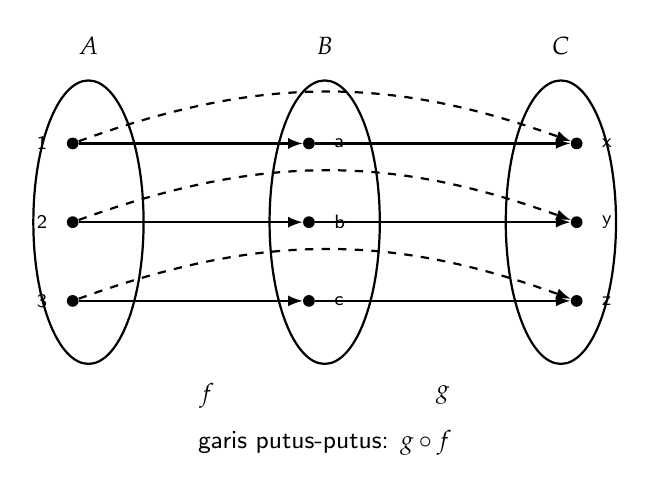
\begin{tikzpicture}[
			dot/.style={circle, fill=black, inner sep=1.5pt},
			elbl/.style={font=\scriptsize\sffamily},
			hdr/.style={font=\sffamily\small, anchor=south}
		]
		\draw[thick] (-3, 0) ellipse (0.7 and 1.8);
		\draw[thick] (0, 0) ellipse (0.7 and 1.8);
		\draw[thick] (3, 0) ellipse (0.7 and 1.8);
		\node[hdr] at (-3, 2.0) {$A$};
		\node[hdr] at (0, 2.0) {$B$};
		\node[hdr] at (3, 2.0) {$C$};

		\node[dot] (a1) at (-3.2, 1.0) {};
		\node[dot] (a2) at (-3.2, 0) {};
		\node[dot] (a3) at (-3.2, -1.0) {};
		\node[elbl, anchor=east] at (-3.4, 1.0) {1};
		\node[elbl, anchor=east] at (-3.4, 0) {2};
		\node[elbl, anchor=east] at (-3.4, -1.0) {3};

		\node[dot] (b1) at (-0.2, 1.0) {};
		\node[dot] (b2) at (-0.2, 0) {};
		\node[dot] (b3) at (-0.2, -1.0) {};
		\node[elbl, anchor=west] at (0, 1.0) {a};
		\node[elbl, anchor=west] at (0, 0) {b};
		\node[elbl, anchor=west] at (0, -1.0) {c};

		\node[dot] (c1) at (3.2, 1.0) {};
		\node[dot] (c2) at (3.2, 0) {};
		\node[dot] (c3) at (3.2, -1.0) {};
		\node[elbl, anchor=west] at (3.4, 1.0) {x};
		\node[elbl, anchor=west] at (3.4, 0) {y};
		\node[elbl, anchor=west] at (3.4, -1.0) {z};

		\draw[thick, -latex] (a1) -- (b1);
		\draw[thick, -latex] (a2) -- (b2);
		\draw[thick, -latex] (a3) -- (b3);
		\draw[thick, -latex] (b1) -- (c1);
		\draw[thick, -latex] (b2) -- (c2);
		\draw[thick, -latex] (b3) -- (c3);

		\draw[thick, dashed, -latex, bend left=20] (a1) to (c1);
		\draw[thick, dashed, -latex, bend left=20] (a2) to (c2);
		\draw[thick, dashed, -latex, bend left=20] (a3) to (c3);

		\node[font=\sffamily\small] at (-1.5, -2.2) {$f$};
		\node[font=\sffamily\small] at (1.5, -2.2) {$g$};
		\node[font=\sffamily\small] at (0, -2.8) {garis putus-putus: $g \circ f$};
	\end{tikzpicture}
	\caption{Komposisi $g \circ f$: rantai dari $A$ ke $C$ melewati $B$.}
	\label{fig:komposisi}
\end{figure}

Cara membaca Gambar~\ref{fig:komposisi}: gambar ini menampilkan tiga elips berderet dari kiri ke kanan, berlabel $A$, $B$, dan $C$. Masing-masing berisi tiga titik. Panah penuh dari $A$ ke $B$ adalah $f$, dan panah penuh dari $B$ ke $C$ adalah $g$. Panah putus-putus dari $A$ langsung ke $C$ adalah $g \circ f$, jalan pintas yang melewati $B$. Di bawah gambar tertulis label $f$ di kiri, $g$ di kanan, dan "garis putus-putus: $g \circ f$" di tengah. Inti pesan gambar ini adalah komposisi memendekkan rantai dua langkah menjadi satu langkah, dan urutan tetap penting karena $f$ dikerjakan lebih dulu.

\subsection{Kalau Salah: Urutan Komposisi Dibaca Terbalik}

Kesalahan paling sering adalah membaca $g \circ f$ dari kiri ke kanan, sehingga mengira $f$ dikerjakan setelah $g$. Padahal notasi $g \circ f$ dibaca dari kanan ke kiri, yaitu $f$ dulu, baru $g$.

Akibatnya, jika domain dan kodomain tidak simetris, pengembang akan mencoba menyambung $g$ dulu baru $f$, padahal hasil $g$ mungkin tidak berada di domain $f$. Komposisi tidak terdefinisi.

Cara aman adalah membaca notasi dengan suara. "$g$ setelah $f$" berarti kerjakan $f$ dulu. Kalau dibaca "$g$ komposisi $f$", kata "komposisi" tetap menandakan urutan yang sama.

\subsection{Mengapa Komposisi Penting}

Di pemrograman, komposisi muncul sebagai pemanggilan bersarang. Contoh: \texttt{hash(bersihkan(teks))}. Fungsi \texttt{bersihkan} mengubah teks menjadi teks yang lebih rapi, dan fungsi \texttt{hash} mengubah teks rapi menjadi sidik jari. Rantai ini adalah komposisi $hash \circ bersihkan$.

Jika \texttt{bersihkan} tidak mengembalikan teks, melainkan mengembalikan bilangan, komposisi tidak terdefinisi. Itulah mengapa syarat komposisi penting: hasil fungsi pertama harus kompatibel dengan masukan fungsi kedua \cite{kleppmann}.

\subsection{Ringkasan}

Tabel~\ref{tab:komposisi-fungsi} merangkum komposisi.

\begin{table}[H]
	\centering
	\caption{Ringkasan komposisi fungsi.}
	\label{tab:komposisi-fungsi}
	\small
	\begin{tabularx}{\textwidth}{l X}
		\toprule
		Aspek           & Isi                                          \\
		\midrule
		Notasi          & $(g \circ f)(x)=g(f(x))$                     \\
		Urutan baca     & dari kanan ke kiri ($f$ dulu)                \\
		Syarat          & jelajah $f$ harus di dalam domain $g$        \\
		Contoh          & $f(x)=3x+1$, $g(x)=x^2$, $(g \circ f)(2)=49$ \\
		Tidak komutatif & $(g \circ f)(2) \ne (f \circ g)(2)$          \\
		Padanan program & \texttt{hash(bersihkan(teks))}               \\
		\bottomrule
	\end{tabularx}
\end{table}

\section{Fungsi Khusus}

\subsection{Lantai dan Langit-langit}

Fungsi lantai $\lfloor x \rfloor$ membulatkan $x$ ke bawah ke bilangan bulat terdekat. Contoh: $\lfloor 3{,}7 \rfloor=3$ dan $\lfloor -1{,}2 \rfloor=-2$. Fungsi langit-langit $\lceil x \rceil$ membulatkan $x$ ke atas. Contoh: $\lceil 3{,}2 \rceil=4$ dan $\lceil -1{,}2 \rceil=-1$.

Kedua fungsi itu sering dipakai di perangkat lunak untuk menghitung jumlah halaman. Jika satu halaman menampung 10 data dan ada 47 data, jumlah halaman adalah $\lceil 47/10 \rceil=5$ halaman. Jika ada 100 data, jumlah halaman adalah $\lceil 100/10 \rceil=10$. Jika ada 101 data, jumlah halaman adalah $\lceil 101/10 \rceil=11$. Perhatikan Gambar~\ref{fig:lantai-langit}.

\begin{figure}[H]
	\centering
	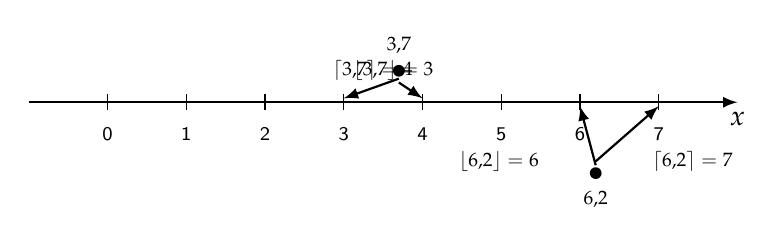
\begin{tikzpicture}[
			pt/.style={circle, fill=black, inner sep=1.5pt},
			lbl/.style={font=\scriptsize\sffamily}
		]
		\draw[thick, -latex] (-1, 0) -- (8, 0) node[below] {$x$};
		\foreach \x/\v in {0/0, 1/1, 2/2, 3/3, 4/4, 5/5, 6/6, 7/7} {
				\draw (\x, 0.1) -- (\x, -0.1);
				\node[lbl] at (\x, -0.4) {\v};
			}

		\node[pt] (p1) at (3.7, 0.4) {};
		\node[lbl, above] at (3.7, 0.5) {$3{,}7$};
		\draw[thick, -latex] (3.7, 0.3) -- (3, 0.05);
		\node[lbl, above right] at (3.0, 0.15) {$\lfloor 3{,}7 \rfloor=3$};

		\draw[thick, -latex] (3.7, 0.25) -- (4, 0.05);
		\node[lbl, above left] at (4.0, 0.15) {$\lceil 3{,}7 \rceil=4$};

		\node[pt] (p2) at (6.2, -0.9) {};
		\node[lbl, below] at (6.2, -1.0) {$6{,}2$};
		\draw[thick, -latex] (6.2, -0.8) -- (6, -0.05);
		\node[lbl, below left] at (5.6, -0.5) {$\lfloor 6{,}2 \rfloor=6$};
		\draw[thick, -latex] (6.2, -0.75) -- (7, -0.05);
		\node[lbl, below right] at (6.8, -0.5) {$\lceil 6{,}2 \rceil=7$};
	\end{tikzpicture}
	\caption{Fungsi lantai dan langit-langit pada garis bilangan.}
	\label{fig:lantai-langit}
\end{figure}

Cara membaca Gambar~\ref{fig:lantai-langit}: gambar ini menampilkan garis bilangan horizontal berlabel $x$ dengan tanda di setiap bilangan bulat 0 sampai 7. Dua titik ditandai. Titik pertama di 3,7 dengan dua panah: panah ke kiri menuju 3 mewakili lantai, panah ke kanan menuju 4 mewakili langit-langit. Titik kedua di 6,2 dengan dua panah serupa: panah ke kiri menuju 6 mewakili lantai, panah ke kanan menuju 7 mewakili langit-langit. Inti pesan gambar ini adalah lantai dan langit-langit mengapit bilangan ke dua bilangan bulat terdekat.

\subsection{Modulo}

Modulo $a \bmod n$ adalah sisa pembagian $a$ oleh $n$. Jika $a=n \cdot q+r$ dengan $q$ adalah hasil bagi dan $r$ adalah sisa, maka $r=a \bmod n$. Contoh: $17 \bmod 5=2$ karena $17=5 \cdot 3+2$. Contoh lain: $(22+5) \bmod 24=3$ karena $27=24 \cdot 1+3$.

Modulo dipakai di pemrograman untuk perhitungan siklik. Jam dinding memakai modulo 12 atau 24. Kalender memakai modulo 7 untuk menentukan hari. Sandi geser memakai modulo 26 untuk memutar huruf \cite{rosen}.

Perhatian khusus: di matematika, $-7 \bmod 3=2$. Di bahasa C dan Java, $-7 \bmod 3=-1$. Perbedaan ini berasal dari cara masing-masing menafsirkan sisa pembagian ketika hasil bagi negatif. Di Python, $-7 \bmod 3=2$ seperti matematika.

\subsection{Faktorial}

Faktorial $n!$ adalah hasil kali $n \cdot (n-1) \cdot (n-2) \cdots 1$, dengan $0!=1$. Contoh: $5!=5 \cdot 4 \cdot 3 \cdot 2 \cdot 1=120$. Definisi $0!=1$ dipakai agar rumus kombinatorial tetap konsisten.

Faktorial tumbuh sangat cepat. $10!=3{.}628{.}800$ dan $20! \approx 2{,}43 \times 10^{18}$. Di pemrograman, faktorial di atas 20 tidak muat di bilangan bulat 64-bit, sehingga memerlukan bilangan besar khusus.

\subsection{Ringkasan}

Tabel~\ref{tab:fungsi-khusus} merangkum fungsi khusus.

\begin{table}[H]
	\centering
	\caption{Ringkasan fungsi khusus.}
	\label{tab:fungsi-khusus}
	\small
	\begin{tabularx}{\textwidth}{l X X}
		\toprule
		Fungsi                          & Arti                    & Contoh                    \\
		\midrule
		Lantai $\lfloor x \rfloor$      & pembulatan ke bawah     & $\lfloor 3{,}7 \rfloor=3$ \\
		Langit-langit $\lceil x \rceil$ & pembulatan ke atas      & $\lceil 3{,}2 \rceil=4$   \\
		Modulo $a \bmod n$              & sisa bagi               & $17 \bmod 5=2$            \\
		Faktorial $n!$                  & hasil kali 1 sampai $n$ & $5!=120$                  \\
		\bottomrule
	\end{tabularx}
\end{table}

\section{Fungsi Rekursif}

\subsection{Analogi: Boneka Rusia}

Bayangkan boneka Rusia berlapis. Setiap boneka berisi boneka yang lebih kecil. Untuk menghitung total boneka, kita membuka boneka terbesar, menghitung satu, lalu membuka boneka di dalamnya, menghitung satu lagi, dan seterusnya sampai boneka terkecil yang tidak berisi apa-apa.

Boneka terkecil adalah basis. Membuka boneka besar dan menghitung sisanya adalah rekurens. Tanpa basis, kita akan membuka boneka tanpa henti.

\subsection{Basis dan Rekurens}

Fungsi rekursif adalah fungsi yang memanggil dirinya sendiri. Setiap fungsi rekursif wajib memiliki dua bagian. Basis adalah kondisi yang menghentikan pemanggilan. Rekurens adalah langkah yang memecah masalah menjadi masalah lebih kecil dan memanggil fungsi lagi dengan masalah yang lebih kecil itu \cite{rosen}.

Tanpa basis, pemanggilan tidak pernah berhenti. Tanpa rekurens, fungsi tidak pernah menyelesaikan masalah yang lebih besar dari basis.

\subsection{Faktorial Rekursif}

Definisi faktorial rekursif: $n!=n \cdot (n-1)!$ untuk $n \ge 1$, dengan $0!=1$. Basisnya adalah $0!=1$. Rekurensnya adalah $n!=n \cdot (n-1)!$.

Untuk menghitung $4!$, telusuri langkahnya. $4!=4 \cdot 3!$. Hitung $3!=3 \cdot 2!$. Hitung $2!=2 \cdot 1!$. Hitung $1!=1 \cdot 0!$. Hitung $0!=1$ (basis). Kemudian kembali ke atas: $1!=1 \cdot 1=1$, $2!=2 \cdot 1=2$, $3!=3 \cdot 2=6$, $4!=4 \cdot 6=24$. Perhatikan Gambar~\ref{fig:faktorial-pohon}.

\begin{figure}[H]
	\centering
	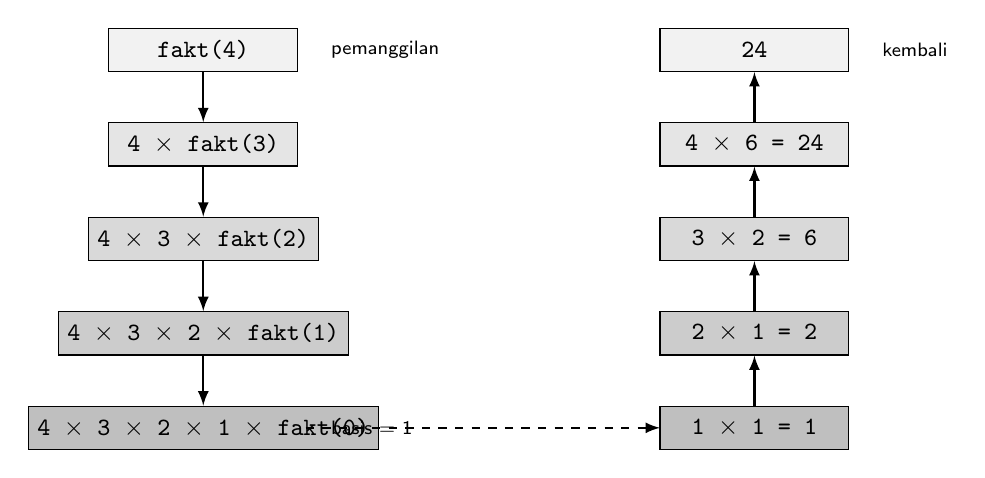
\begin{tikzpicture}[
			box/.style={rectangle, draw=black, minimum width=2.4cm, minimum height=0.55cm, align=center, font=\ttfamily\small},
			lbl/.style={font=\scriptsize\sffamily}
		]
		\node[box, fill=black!5] (f4) at (0, 4) {fakt(4)};
		\node[box, fill=black!10] (f3) at (0, 2.8) {4 $\times$ fakt(3)};
		\node[box, fill=black!15] (f2) at (0, 1.6) {4 $\times$ 3 $\times$ fakt(2)};
		\node[box, fill=black!20] (f1) at (0, 0.4) {4 $\times$ 3 $\times$ 2 $\times$ fakt(1)};
		\node[box, fill=black!25] (f0) at (0, -0.8) {4 $\times$ 3 $\times$ 2 $\times$ 1 $\times$ fakt(0)};

		\draw[thick, -latex] (f4) -- (f3);
		\draw[thick, -latex] (f3) -- (f2);
		\draw[thick, -latex] (f2) -- (f1);
		\draw[thick, -latex] (f1) -- (f0);

		\node[lbl, anchor=west] at (1.5, 4) {pemanggilan};
		\node[lbl, anchor=west] at (1.5, -0.8) {basis = 1};

		\node[box, fill=black!5] (r4) at (7, 4) {24};
		\node[box, fill=black!10] (r3) at (7, 2.8) {4 $\times$ 6 = 24};
		\node[box, fill=black!15] (r2) at (7, 1.6) {3 $\times$ 2 = 6};
		\node[box, fill=black!20] (r1) at (7, 0.4) {2 $\times$ 1 = 2};
		\node[box, fill=black!25] (r0) at (7, -0.8) {1 $\times$ 1 = 1};

		\draw[thick, -latex] (r0) -- (r1);
		\draw[thick, -latex] (r1) -- (r2);
		\draw[thick, -latex] (r2) -- (r3);
		\draw[thick, -latex] (r3) -- (r4);

		\node[lbl, anchor=west] at (8.5, 4) {kembali};
		\draw[thick, dashed, -latex] (1.3, -0.8) -- (5.8, -0.8);
	\end{tikzpicture}
	\caption{Pohon pemanggilan rekursif untuk $4!$: turun sampai basis, lalu naik mengalikan hasil.}
	\label{fig:faktorial-pohon}
\end{figure}

Cara membaca Gambar~\ref{fig:faktorial-pohon}: gambar ini menampilkan dua kolom kotak. Kolom kiri adalah jalur pemanggilan, dari atas ke bawah, dimulai dari \texttt{fakt(4)} lalu berangsur-angsur menyertakan perkalian yang menunggu sampai mencapai \texttt{fakt(0)} di dasar. Kotak paling bawah adalah basis dengan nilai 1. Kolom kanan adalah jalur kembali, dari bawah ke atas, dimulai dari hasil basis 1, lalu mengalikan dengan 1, 2, 3, 4 sampai kembali ke hasil akhir 24 di atas. Garis putus-putus di dasar menghubungkan kolom kiri dan kolom kanan, menandakan titik balik. Inti pesan gambar ini adalah rekursi berjalan ke bawah sampai basis, lalu hasilnya dikalikan sambil naik kembali ke atas.

\subsection{Fibonacci Rekursif}

Fibonacci didefinisikan oleh $F(0)=0$, $F(1)=1$, dan $F(n)=F(n-1)+F(n-2)$ untuk $n \ge 2$. Barisannya adalah 0, 1, 1, 2, 3, 5, 8, dan seterusnya.

Untuk menghitung $F(4)$, pemanggilan bercabang. $F(4)$ memanggil $F(3)$ dan $F(2)$. $F(3)$ memanggil $F(2)$ dan $F(1)$. $F(2)$ memanggil $F(1)$ dan $F(0)$. Perhatikan bahwa $F(2)$ dihitung dua kali, dan $F(1)$ dihitung tiga kali. Perhatikan Gambar~\ref{fig:fibonacci-pohon}.

\begin{figure}[H]
	\centering
	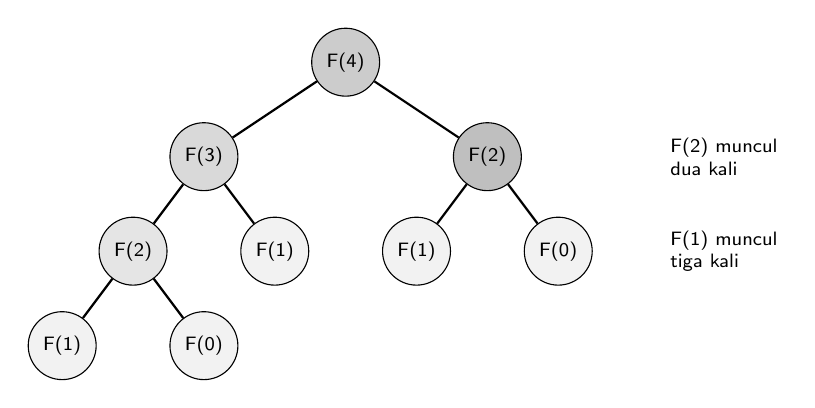
\begin{tikzpicture}[
			node/.style={circle, draw=black, minimum size=0.7cm, font=\scriptsize\sffamily}
		]
		\node[node, fill=black!20] (f4) at (0, 3) {F(4)};
		\node[node, fill=black!15] (f3) at (-1.8, 1.8) {F(3)};
		\node[node, fill=black!25] (f2a) at (1.8, 1.8) {F(2)};
		\node[node, fill=black!10] (f2b) at (-2.7, 0.6) {F(2)};
		\node[node, fill=black!5] (f1a) at (-0.9, 0.6) {F(1)};
		\node[node, fill=black!5] (f1b) at (0.9, 0.6) {F(1)};
		\node[node, fill=black!5] (f0a) at (2.7, 0.6) {F(0)};
		\node[node, fill=black!5] (f1c) at (-3.6, -0.6) {F(1)};
		\node[node, fill=black!5] (f0b) at (-1.8, -0.6) {F(0)};

		\draw[thick] (f4) -- (f3);
		\draw[thick] (f4) -- (f2a);
		\draw[thick] (f3) -- (f2b);
		\draw[thick] (f3) -- (f1a);
		\draw[thick] (f2a) -- (f1b);
		\draw[thick] (f2a) -- (f0a);
		\draw[thick] (f2b) -- (f1c);
		\draw[thick] (f2b) -- (f0b);

		\node[font=\scriptsize\sffamily, align=left, anchor=west] at (4, 1.8) {F(2) muncul\\dua kali};
		\node[font=\scriptsize\sffamily, align=left, anchor=west] at (4, 0.6) {F(1) muncul\\tiga kali};
	\end{tikzpicture}
	\caption{Pohon pemanggilan Fibonacci $F(4)$ dengan hitungan berulang.}
	\label{fig:fibonacci-pohon}
\end{figure}

Cara membaca Gambar~\ref{fig:fibonacci-pohon}: gambar ini menampilkan pohon dengan $F(4)$ di puncak. Dari $F(4)$ keluar dua cabang ke $F(3)$ di kiri dan $F(2)$ di kanan. Dari $F(3)$ keluar dua cabang ke $F(2)$ dan $F(1)$. Dari $F(2)$ yang kanan keluar dua cabang ke $F(1)$ dan $F(0)$. Dari $F(2)$ yang kiri keluar dua cabang ke $F(1)$ dan $F(0)$. Di sebelah kanan gambar ada dua keterangan: "F(2) muncul dua kali" dan "F(1) muncul tiga kali". Inti pesan gambar ini adalah rekursi Fibonacci tanpa optimasi menghitung ulang submasalah yang sama, sehingga jumlah pemanggilan tumbuh sangat cepat.

\subsection{Kalau Salah: Rekursi Tanpa Basis}

Kesalahan paling sering adalah menulis fungsi rekursif tanpa basis. Kode seperti \texttt{fakt(n)~=~n~*~fakt(n-1)} tanpa kondisi berhenti akan memanggil dirinya sendiri tanpa henti sampai tumpukan panggilan penuh, dan program berhenti dengan galat stack overflow.

Basis adalah satu-satunya yang menghentikan rekursi. Tanpanya, rekursi bukan algoritma, tetapi bencana.

\subsection{Kalau Salah: Rekursi Fibonacci Tanpa Memo}

Kesalahan kedua adalah memakai rekursi Fibonacci apa adanya untuk nilai besar. Untuk $F(40)$, rekursi biasa memerlukan sekitar 300 juta pemanggilan, sedangkan loop sederhana hanya memerlukan 40 langkah. Solusinya adalah menyimpan hasil yang sudah dihitung di dalam tabel memoisasi, sehingga setiap submasalah hanya dihitung sekali \cite{kleppmann}.

\subsection{Ringkasan}

Tabel~\ref{tab:rekursi} merangkum fungsi rekursif.

\begin{table}[H]
	\centering
	\caption{Ringkasan fungsi rekursif.}
	\label{tab:rekursi}
	\small
	\begin{tabularx}{\textwidth}{l X X}
		\toprule
		Aspek       & Basis                   & Rekurens                          \\
		\midrule
		Faktorial   & $0!=1$                  & $n!=n \cdot (n-1)!$               \\
		Deret       & $S(0)=0$                & $S(n)=n+S(n-1)$                   \\
		Fibonacci   & $F(0)=0$, $F(1)=1$      & $F(n)=F(n-1)+F(n-2)$              \\
		Tanpa basis & pemanggilan tidak henti & stack overflow                    \\
		Optimasi    & memoisasi               & setiap submasalah dihitung sekali \\
		\bottomrule
	\end{tabularx}
\end{table}

\section{Sintesis Seluruh Konsep}

Tabel~\ref{tab:sintesis} menyandingkan seluruh konsep dalam satu pandangan.

\begin{table}[H]
	\centering
	\caption{Sintesis konsep fungsi untuk rekayasa perangkat lunak.}
	\label{tab:sintesis}
	\footnotesize
	\begin{tabularx}{\textwidth}{l X X X}
		\toprule
		Lapisan   & Pertanyaan                                 & Alat                          & Contoh penerapan               \\
		\midrule
		Bentuk    & apakah relasi punya satu hasil per masukan & definisi fungsi               & kamus Python                   \\
		Periksa   & berapa hasil per masukan                   & tiga pertanyaan               & validasi input                 \\
		Sifat     & apakah hasil berbeda dan semua terpakai    & injektif, surjektif, bijektif & NIM unik, enkripsi             \\
		Invers    & bisakah hasil dilacak balik                & $f^{-1}$                      & dekripsi                       \\
		Komposisi & bisakah dua fungsi disambung               & $g \circ f$                   & \texttt{hash(bersihkan(teks))} \\
		Khusus    & pembulatan, sisa, hasil kali               & lantai, modulo, faktorial     & paginasi, jam, kombinasi       \\
		Rekursif  & fungsi memanggil dirinya sendiri           & basis dan rekurens            & pohon pencarian                \\
		\bottomrule
	\end{tabularx}
\end{table}

Sintesis dari Tabel~\ref{tab:sintesis} adalah satu pola berpikir. Masalah diubah menjadi fungsi dengan domain dan kodomain yang jelas. Sifatnya diperiksa untuk memastikan hasil dapat dilacak balik. Komposisi dipakai untuk menyambung dua fungsi. Fungsi khusus dipakai untuk membulatkan dan menghitung sisa. Rekursi dipakai untuk masalah yang bisa dipecah menjadi masalah lebih kecil. Pola ini berlaku dari validasi input sampai algoritma pencarian.

\section{Studi Kasus: Sandi Geser}

\subsection{Langkah 1: Definisikan Himpunan}

Huruf alfabet Inggris diberi nomor: A=0, B=1, C=2, sampai Z=25. Himpunan asal dan himpunan tujuan adalah sama, yaitu $\{0,1,\ldots,25\}$. Keduanya berisi 26 elemen.

\subsection{Langkah 2: Definisikan Fungsi Geser}

Fungsi geser didefinisikan oleh $\text{geser}(x)=(x+3) \bmod 26$. Untuk setiap huruf bernomor $x$, geser menambahkan 3 lalu mengambil sisa bagi 26. Jika hasilnya melewati 25, ia kembali ke 0. Perhatikan Gambar~\ref{fig:sandi-geser}.

\begin{figure}[H]
	\centering
	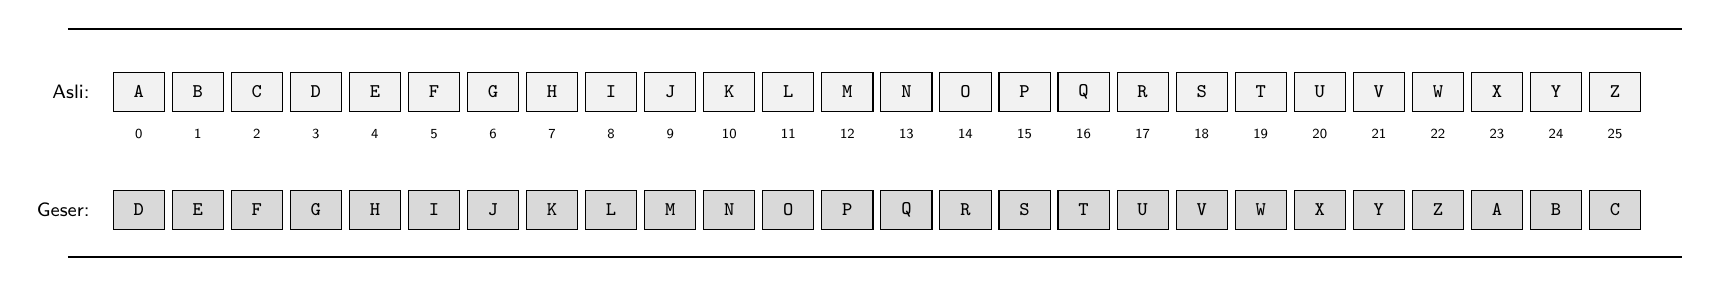
\begin{tikzpicture}[
			cell/.style={rectangle, draw=black, minimum width=0.65cm, minimum height=0.5cm, align=center, font=\scriptsize\ttfamily},
			lbl/.style={font=\scriptsize\sffamily, align=center}
		]
		\node[lbl, anchor=east] at (-0.5, 1.5) {Asli:};
		\foreach \letter [count=\i] in {A,B,C,D,E,F,G,H,I,J,K,L,M,N,O,P,Q,R,S,T,U,V,W,X,Y,Z} {
				\node[cell, fill=black!5] at (\i*0.75 - 0.75, 1.5) {\letter};
				\node[font=\tiny\sffamily, anchor=north] at (\i*0.75 - 0.75, 1.15) {\number\numexpr\i-1\relax};
			}

		\node[lbl, anchor=east] at (-0.5, 0) {Geser:};
		\foreach \letter [count=\i] in {D,E,F,G,H,I,J,K,L,M,N,O,P,Q,R,S,T,U,V,W,X,Y,Z,A,B,C} {
				\node[cell, fill=black!15] at (\i*0.75 - 0.75, 0) {\letter};
			}

		\draw[thick] (-0.9, 2.3) -- (19.6, 2.3);
		\draw[thick] (-0.9, -0.6) -- (19.6, -0.6);
	\end{tikzpicture}
	\caption{Sandi geser dengan pergeseran 3: A menjadi D, B menjadi E, sampai X, Y, Z kembali ke A, B, C.}
	\label{fig:sandi-geser}
\end{figure}

Cara membaca Gambar~\ref{fig:sandi-geser}: gambar ini menampilkan dua baris kotak huruf. Baris atas berlabel "Asli" berisi huruf A sampai Z berurutan, dengan angka 0 sampai 25 di bawah setiap huruf. Baris bawah berlabel "Geser" berisi huruf yang sama tetapi dimulai dari D. Huruf A di baris atas berpasangan dengan D di baris bawah, B dengan E, C dengan F, dan seterusnya. Tiga huruf terakhir di baris atas X, Y, Z berpasangan dengan A, B, C di baris bawah karena modulo 26 memutar kembali ke awal. Inti pesan gambar ini adalah sandi geser memutar alfabet dan modulo 26 memastikan tidak ada huruf yang keluar dari rentang.

\subsection{Langkah 3: Periksa Bijektif}

Fungsi geser adalah bijektif. Setiap huruf punya tepat satu hasil, dan setiap hasil berasal dari tepat satu huruf. Buktinya sederhana: jika $\text{geser}(x_1)=\text{geser}(x_2)$, maka $(x_1+3) \bmod 26=(x_2+3) \bmod 26$, sehingga $x_1 \equiv x_2 \pmod{26}$. Karena $x_1$ dan $x_2$ keduanya di rentang 0 sampai 25, maka $x_1=x_2$. Ini membuktikan injektif. Surjektif dibuktikan dengan menunjukkan setiap $y$ berasal dari $(y-3) \bmod 26$.

\subsection{Langkah 4: Enkripsi "RPL"}

Huruf R bernomor 17, P bernomor 15, L bernomor 11. Terapkan fungsi geser ke setiap huruf. R menjadi $(17+3) \bmod 26=20$, yaitu U. P menjadi $(15+3) \bmod 26=18$, yaitu S. L menjadi $(11+3) \bmod 26=14$, yaitu O. Hasil enkripsi "RPL" adalah "USO".

\subsection{Langkah 5: Definisikan Invers}

Invers fungsi geser adalah $\text{geser}^{-1}(x)=(x-3) \bmod 26$. Karena modulo tidak mengizinkan pengurangan negatif, rumus alternatifnya adalah $(x+23) \bmod 26$. Kedua rumus memberi hasil yang sama, tetapi rumus kedua lebih aman di bahasa pemrograman yang tidak mendukung modulo negatif sesuai matematika.

\subsection{Langkah 6: Dekripsi "USO"}

Huruf U bernomor 20, S bernomor 18, O bernomor 14. Terapkan invers. U menjadi $(20-3) \bmod 26=17$, yaitu R. S menjadi $(18-3) \bmod 26=15$, yaitu P. O menjadi $(14-3) \bmod 26=11$, yaitu L. Hasil dekripsi "USO" adalah "RPL", cocok dengan pesan asli.

\subsection{Langkah 7: Komposisi Dua Geser}

Geser dengan pergeseran 3 dikomposisikan dengan geser pergeseran 3 lagi. Hasilnya adalah geser dengan pergeseran 6. Buktinya: $(\text{geser} \circ \text{geser})(x)=((x+3) \bmod 26+3) \bmod 26=(x+6) \bmod 26$. Komposisi sandi geser bersifat komutatif, artinya urutan tidak berpengaruh, karena operasi penjumlahan modulo bersifat komutatif.

\subsection{Langkah 8: Verifikasi}

Untuk memverifikasi, enkripsi lalu dekripsi harus mengembalikan pesan asli. Enkripsi "RPL" menghasilkan "USO". Dekripsi "USO" menghasilkan "RPL". Hasilnya cocok. Inilah sifat bijektif yang menjamin enkripsi dan dekripsi selalu berpasangan. Alur lengkap studi kasus ditunjukkan pada Gambar~\ref{fig:alur-sandi}.

\begin{figure}[H]
	\centering
	\begin{tikzpicture}[
			step/.style={rectangle, draw=black, thick, fill=black!5, text width=9cm, align=left, minimum height=0.7cm, font=\sffamily\small, inner sep=8pt},
			line/.style={draw, thick, -latex}
		]
		\node[step] (s1) {\textbf{1.} Definisikan alfabet 0--25};
		\node[step, below=0.25cm of s1] (s2) {\textbf{2.} Definisikan $\text{geser}(x)=(x+3) \bmod 26$};
		\node[step, below=0.25cm of s2] (s3) {\textbf{3.} Periksa bijektif};
		\node[step, below=0.25cm of s3] (s4) {\textbf{4.} Enkripsi "RPL" menjadi "USO"};
		\node[step, below=0.25cm of s4] (s5) {\textbf{5.} Definisikan $\text{geser}^{-1}(x)=(x-3) \bmod 26$};
		\node[step, below=0.25cm of s5] (s6) {\textbf{6.} Dekripsi "USO" menjadi "RPL"};
		\node[step, below=0.25cm of s6] (s7) {\textbf{7.} Komposisi dua geser = geser 6};
		\node[step, below=0.25cm of s7] (s8) {\textbf{8.} Verifikasi bolak-balik};
		\draw[line] (s1) -- (s2);
		\draw[line] (s2) -- (s3);
		\draw[line] (s3) -- (s4);
		\draw[line] (s4) -- (s5);
		\draw[line] (s5) -- (s6);
		\draw[line] (s6) -- (s7);
		\draw[line] (s7) -- (s8);
	\end{tikzpicture}
	\caption{Alur delapan langkah studi kasus sandi geser.}
	\label{fig:alur-sandi}
\end{figure}

Cara membaca Gambar~\ref{fig:alur-sandi}: gambar ini menampilkan delapan kotak persegi panjang tersusun dari atas ke bawah. Setiap kotak berisi satu langkah, diawali angka tebal. Kotak pertama "Definisikan alfabet 0--25". Kotak kedua "Definisikan geser(x)=(x+3) mod 26". Kotak ketiga "Periksa bijektif". Kotak keempat "Enkripsi RPL menjadi USO". Kotak kelima "Definisikan geser^-1(x)=(x-3) mod 26". Kotak keenam "Dekripsi USO menjadi RPL". Kotak ketujuh "Komposisi dua geser = geser 6". Kotak kedelapan "Verifikasi bolak-balik". Setiap kotak dihubungkan ke kotak berikutnya oleh panah pendek yang mengarah ke bawah. Latar kotak abu-abu sangat muda. Inti pesan gambar ini adalah proses enkripsi dan dekripsi berjalan berurutan dari definisi sampai verifikasi.

\begin{table}[H]
	\centering
	\caption{Ringkasan hasil studi kasus sandi geser.}
	\label{tab:studi-sandi}
	\small
	\begin{tabularx}{\textwidth}{l X l}
		\toprule
		Langkah & Operasi                & Hasil             \\
		\midrule
		1       & alfabet 0--25          & 26 elemen         \\
		2       & $\text{geser}(x)$      & $(x+3) \bmod 26$  \\
		3       & bijektif               & terbukti          \\
		4       & RPL                    & USO               \\
		5       & $\text{geser}^{-1}(x)$ & $(x-3) \bmod 26$  \\
		6       & USO                    & RPL               \\
		7       & komposisi              & geser 6           \\
		8       & verifikasi             & cocok bolak-balik \\
		\bottomrule
	\end{tabularx}
\end{table}

\section{Merancang Kasus Uji}

\subsection{Mengapa Kasus Uji Perlu Dirancang}

Fungsi yang benar bukan fungsi yang berjalan sekali tanpa galat. Fungsi yang benar adalah fungsi yang berjalan benar pada semua masukan yang mungkin. Untuk membuktikan itu, kita tidak bisa mencoba semua masukan satu per satu, karena jumlahnya bisa tak terhingga. Yang bisa dilakukan adalah memilih beberapa kasus yang mewakili setiap jenis masukan.

Empat jenis kasus uji yang wajib ada. Kasus normal menguji masukan yang biasa. Kasus batas menguji masukan di tepi rentang. Kasus nol menguji masukan tanpa isi. Kasus di luar daerah asal menguji masukan yang tidak sah.

\subsection{Contoh Kasus Uji}

Fungsi yang diuji adalah $jumlah\_halaman(total, ukuran)=\lceil total/ukuran \rceil$. Tabel~\ref{tab:kasus-uji} memuat kasus ujinya.

\begin{table}[H]
	\centering
	\caption{Kasus uji untuk fungsi jumlah halaman.}
	\label{tab:kasus-uji}
	\small
	\begin{tabularx}{\textwidth}{l X l X}
		\toprule
		Jenis kasus           & Masukan $(total, ukuran)$ & Hasil & Alasan                    \\
		\midrule
		Normal                & $(47, 10)$                & 5     & pembulatan ke atas        \\
		Batas atas tepat      & $(100, 10)$               & 10    & habis dibagi              \\
		Batas atas lebih satu & $(101, 10)$               & 11    & satu lebih dari kelipatan \\
		Batas bawah           & $(0, 10)$                 & 0     & tidak ada data            \\
		Di luar daerah asal   & $(50, 0)$                 & galat & pembagian dengan nol      \\
		\bottomrule
	\end{tabularx}
\end{table}

Kelima kasus itu mencakup seluruh perilaku fungsi. Jika kelima kasus lolos, fungsi bisa dianggap benar pada rentang yang diuji.

\subsection{Mengapa Kasus Uji Diperlukan}

Kasus uji adalah cara membuktikan kebenaran secara empiris. Tanpa kasus uji, pengembang hanya tahu bahwa fungsi berjalan pada satu masukan yang kebetulan dipakai untuk menguji. Dengan kasus uji, pengembang tahu bahwa fungsi berjalan pada semua jenis masukan yang mungkin.

Kasus batas adalah yang paling sering melewatkan bug. Fungsi yang lolos pada 47 tapi gagal pada 100 karena pembulatan salah. Fungsi yang lolos pada 100 tapi gagal pada 101 karena tidak menambahkan halaman ekstra. Pengujian di tepi rentang menemukan bug yang tidak terlihat di tengah.

\section{Kesalahan Umum dan Cara Menghindarinya}

Tabel~\ref{tab:kesalahan} memuat kesalahan yang paling sering muncul saat bekerja dengan fungsi.

\begin{table}[H]
	\centering
	\caption{Kesalahan umum pada penerapan teori fungsi.}
	\label{tab:kesalahan}
	\footnotesize
	\begin{tabularx}{\textwidth}{l X X}
		\toprule
		Kesalahan                                  & Akibat                      & Perbaikan                            \\
		\midrule
		mengira semua relasi adalah fungsi         & dua hasil dianggap satu     & periksa hasil per masukan            \\
		mengira jelajah sama dengan kodomain       & salah menghitung            & hitung hasil yang benar-benar muncul \\
		$f^{-1}(x)$ dikira $1/f(x)$                & hasil numerik salah         & invers membalik pasangan             \\
		invers dihitung tanpa cek bijektif         & invers tidak tunggal        & periksa injektif dan surjektif       \\
		$g \circ f$ dibaca kiri ke kanan           & komposisi tidak terdefinisi & baca dari kanan                      \\
		modulo negatif dianggap seperti matematika & hasil beda di C dan Java    & sesuaikan dengan bahasa              \\
		lantai negatif dianggap seperti positif    & salah pembulatan            & $\lfloor -1{,}2 \rfloor=-2$          \\
		rekursi tanpa basis                        & stack overflow              & tulis kondisi berhenti               \\
		rekursi Fibonacci tanpa memoisasi          & sangat lambat               & simpan hasil                         \\
		kasus uji hanya kasus normal               & bug di tepi terlewat        & tambah kasus batas dan nol           \\
		\bottomrule
	\end{tabularx}
\end{table}

Dua kesalahan yang paling sering adalah mengira $f^{-1}(x)$ sama dengan $1/f(x)$, dan menulis rekursi tanpa basis. Kesalahan pertama membuat hasil numerik berbeda jauh dari jawaban yang benar. Kesalahan kedua membuat program berhenti dengan galat yang tidak informatif. Keduanya dapat dicegah dengan menuliskan definisi fungsi di komentar kode dan memeriksa kasus dasar sebelum menulis rekurens.

\section{Lembar Rujukan Cepat}

Tabel~\ref{tab:rujukan-cepat} adalah lembar rujukan untuk ujian atau kerja.

\begin{table}[H]
	\centering
	\caption{Lembar rujukan cepat teori fungsi.}
	\label{tab:rujukan-cepat}
	\footnotesize
	\begin{tabularx}{\textwidth}{l X}
		\toprule
		Kebutuhan        & Notasi atau langkah                      \\
		\midrule
		definisi fungsi  & setiap masukan tepat satu hasil          \\
		domain           & himpunan semua masukan                   \\
		kodomain         & himpunan tempat hasil boleh berada       \\
		jelajah          & himpunan hasil yang benar-benar muncul   \\
		notasi           & $f:A \to B$, $f(a)=b$                    \\
		injektif         & $f(a_1)=f(a_2) \Rightarrow a_1=a_2$      \\
		surjektif        & setiap $b \in B$ ada $a$ dengan $f(a)=b$ \\
		bijektif         & injektif dan surjektif                   \\
		invers           & $f^{-1}$ ada jika $f$ bijektif           \\
		rumus invers     & $y=f(x)$, cari $x$, tukar $y$ ke $x$     \\
		komposisi        & $(g \circ f)(x)=g(f(x))$                 \\
		urutan komposisi & dari kanan ke kiri ($f$ dulu)            \\
		lantai           & $\lfloor x \rfloor$                      \\
		langit-langit    & $\lceil x \rceil$                        \\
		modulo           & $a \bmod n=r$ dengan $a=nq+r$            \\
		faktorial        & $0!=1$, $n!=n(n-1)!$                     \\
		rekursi basis    & kondisi berhenti                         \\
		rekursi rekurens & langkah pemecahan masalah                \\
		kasus uji        & normal, batas, nol, di luar domain       \\
		\bottomrule
	\end{tabularx}
\end{table}

\section{Kesimpulan}

Modul ini menunjukkan bahwa fungsi adalah alat kerja untuk menjamin satu jawaban pasti untuk setiap masukan. Tiga prinsip penutup adalah sebagai berikut.

\begin{enumerate}
	\item Nyatakan domain dan kodomain sebelum mendefinisikan fungsi. Tanpa batas yang jelas, hasil apa pun bisa tampak sah padahal tidak terdefinisi.
	\item Periksa bijektif sebelum mencari invers. Hanya fungsi bijektif yang punya invers. Fungsi yang tidak bijektif hanya punya balikan relasi, bukan invers fungsi.
	\item Rancang kasus uji di tepi rentang. Bug paling sering muncul di batas, bukan di tengah. Kasus normal, batas, nol, dan di luar domain wajib ada.
\end{enumerate}

Dengan tiga prinsip itu, pembaca dapat mendefinisikan fungsi dengan batas yang jelas, memeriksa sifatnya, mencari inversnya, menyambung dua fungsi, menulis fungsi rekursif, dan merancang kasus uji untuk membuktikan kebenarannya.

\newpage
\section*{Referensi}
\addcontentsline{toc}{section}{Referensi}

\begin{thebibliography}{99}

	\bibitem{rosen}
	Rosen, K. H. (2019).
	\textit{Discrete Mathematics and Its Applications} (8th ed.).
	McGraw-Hill Education.

	\bibitem{munir}
	Munir, R. (2012).
	\textit{Matematika Diskrit}.
	Informatika.

	\bibitem{epp}
	Epp, S. S. (2010).
	\textit{Discrete Mathematics with Applications} (4th ed.).
	Brooks Cole.

	\bibitem{lipschutz}
	Lipschutz, S., \& Lipson, M. (2007).
	\textit{Discrete Mathematics}.
	McGraw-Hill.

	\bibitem{silberschatz}
	Silberschatz, A., Korth, H. F., \& Sudarshan, S. (2019).
	\textit{Database System Concepts} (7th ed.).
	McGraw-Hill Education.

	\bibitem{kleppmann}
	Kleppmann, M. (2017).
	\textit{Designing Data-Intensive Applications}.
	O'Reilly Media.

	\bibitem{sommerville}
	Sommerville, I. (2016).
	\textit{Software Engineering} (10th ed.).
	Pearson.

	\bibitem{cormen}
	Cormen, T. H., Leiserson, C. E., Rivest, R. L., \& Stein, C. (2009).
	\textit{Introduction to Algorithms} (3rd ed.).
	MIT Press.

\end{thebibliography}

\end{document}
